\documentclass[aspectratio=169]{beamer}

% --- PACKAGES ---
\usepackage[utf8]{inputenc}
\usepackage[T5]{fontenc}
\usepackage{lmodern} % Khắc phục lỗi font toán học
\usepackage[vietnamese]{babel}
\usepackage{graphicx}
\usepackage{booktabs}
\usepackage{tabularx}
\usepackage{multicol}
\usepackage{makecell}
\usepackage{adjustbox} % Hỗ trợ co giãn bảng

% --- THEME SETTINGS ---
\usetheme{Madrid}
\usecolortheme{default}
\setbeamertemplate{navigation symbols}{}
\setbeamerfont{caption}{size=\scriptsize} % Chữ caption nhỏ lại

% --- THÔNG TIN TRANG BÌA ---
\title[Dự đoán ý định mua hàng TMĐT]{Mô hình phân lớp hành vi mua hàng của khách \\ trên nền tảng Thương mại điện tử}
\subtitle{Báo cáo Đồ án Học máy}
\author[Hoàng Mạnh Đức]{Sinh viên thực hiện: Hoàng Mạnh Đức \\ MSSV: 20237311}
\institute[Đại học]{Trường Đại học Bách Khoa Hà Nội}
\date{\today}

\begin{document}

% --- SLIDE 1: BÌA ---
\begin{frame}
    \titlepage
\end{frame}

% --- SLIDE 2: MỤC LỤC ---
\begin{frame}{Nội dung trình bày}
    \tableofcontents
\end{frame}

% ==========================================
\section{1. Giới thiệu bài toán}
% ==========================================

\begin{frame}{1.1 Bối cảnh \& Lý do chọn đề tài}
    \textbf{Bối cảnh ngành TMĐT:}
    \begin{itemize}
        \item Lượng truy cập (Traffic) cực cao nhưng tỷ lệ chuyển đổi (Conversion Rate) rất thấp.
        \item Tỷ lệ "bỏ rơi giỏ hàng" (Cart Abandonment Rate) trung bình lên tới gần \textbf{70\%}.
        \item Dữ liệu Nhật ký sự kiện (Event Logs) khổng lồ là mỏ vàng để Học máy "đọc vị" người dùng.
    \end{itemize}
    
    \vspace{0.3cm}
    \textbf{Lý do chọn đề tài:}
    \begin{itemize}
        \item \textbf{Về mặt kinh doanh:} Khắc phục lãng phí do Marketing đại trà, chuyển sang Marketing cá nhân hóa (Targeted Marketing), tối ưu biên lợi nhuận.
        \item \textbf{Về mặt kỹ thuật:} Khai thác dữ liệu sự kiện thô (Raw Event Logs), giải quyết thách thức trích xuất đặc trưng (Feature Engineering) và kiểm soát rò rỉ dữ liệu (Data Leakage).
    \end{itemize}
\end{frame}

\begin{frame}{1.2 Đối tượng sử dụng \& Hỗ trợ ra quyết định}
    Mô hình phục vụ 3 phòng ban cốt lõi:
    \begin{enumerate}
        \item \textbf{Bộ phận Marketing:} Tối ưu hóa ngân sách quảng cáo bám đuôi (Retargeting) và cấp phát Voucher thông minh (Smart Vouchering).
        \item \textbf{Bộ phận CSKH:} Can thiệp thời gian thực (Real-time Intervention) bằng Pop-up Live Chat khi khách hàng dừng lâu ở trang thanh toán.
        \item \textbf{Bộ phận UI/UX:} Tùy biến giao diện (Dynamic UI), tinh gọn nút thanh toán cho khách hàng có ý định mua cao.
    \end{enumerate}
\end{frame}

% ==========================================
\section{2. Mô tả và Tiền xử lý dữ liệu}
% ==========================================

\begin{frame}{2.1 Nguồn dữ liệu \& Từ điển dữ liệu}
    \textbf{Nguồn:} eCommerce Events History in Cosmetics Shop (Kaggle). Quy mô > 20 triệu bản ghi.
    
    \vspace{0.2cm}
    \begin{table}
        \centering
        \caption{Từ điển dữ liệu nguyên bản (Raw Event Logs)}
        \resizebox{\textwidth}{!}{
        \begin{tabular}{lll}
            \toprule
            \textbf{Tên biến} & \textbf{Kiểu dữ liệu} & \textbf{Ý nghĩa} \\
            \midrule
            \texttt{event\_time} & String & Thời điểm xảy ra sự kiện (UTC). \\
            \texttt{event\_type} & String & Loại tương tác: \texttt{view}, \texttt{cart}, \texttt{remove\_from\_cart}, \texttt{purchase}. \\
            \texttt{product\_id} & int64 & Mã định danh sản phẩm. \\
            \texttt{category\_id} / \texttt{category\_code} & int64 / string & Định danh danh mục \& Tên chuỗi phân cấp. \\
            \texttt{brand} & string & Thương hiệu sản phẩm. \\
            \texttt{price} & Float64 & Giá sản phẩm (USD). \\
            \texttt{user\_id} / \texttt{user\_session} & int64 / string & Mã khách hàng \& Mã phiên truy cập. \\
            \bottomrule
        \end{tabular}
        }
    \end{table}
\end{frame}

\begin{frame}{2.2 Kiểm tra chất lượng dữ liệu thô (Phần 1)}
    \begin{columns}
        \begin{column}{0.5\textwidth}
            \textbf{1. Kiểm tra Kiểu dữ liệu (Data Types):}
            \begin{itemize}
                \item Cột \texttt{event\_time} ban đầu được hệ thống đọc dưới dạng chuỗi văn bản (Object).
                \item \textit{Vấn đề:} Cần chuyển đổi sang định dạng \texttt{Datetime} để phục vụ tính toán thời lượng lướt web.
            \end{itemize}
            \begin{center}
                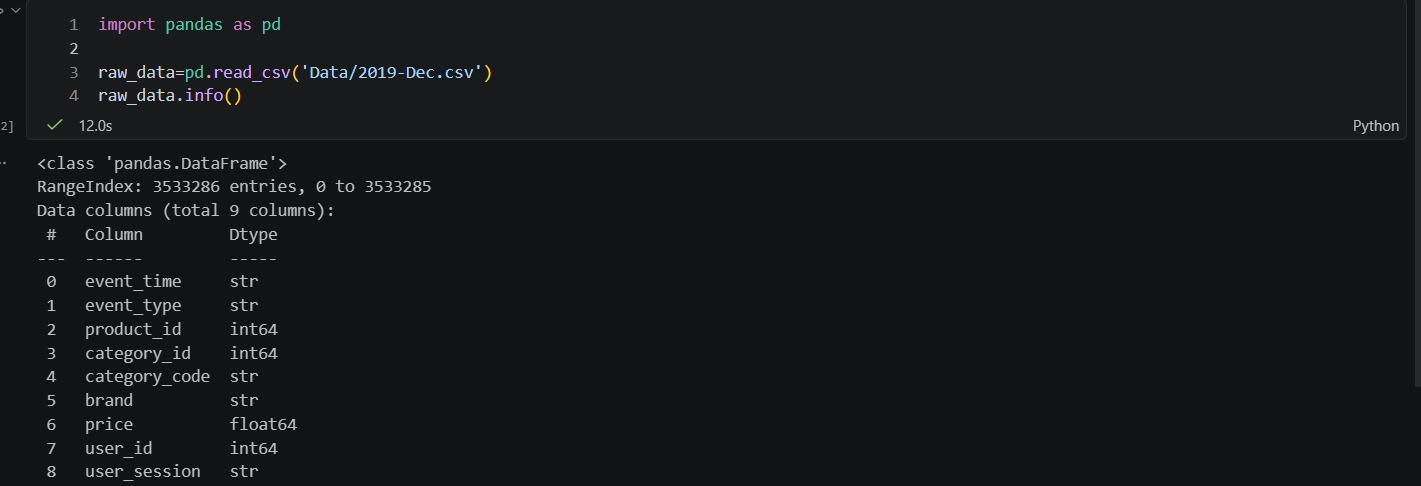
\includegraphics[width=0.9\textwidth]{IMG/Datavalid1.png}
            \end{center}
        \end{column}
        
        \begin{column}{0.5\textwidth}
            \textbf{2. Kiểm tra Dữ liệu thiếu (Missing Values):}
            \begin{itemize}
                \item Các trường giao dịch (session, type, price) đầy 100\%.
                \item \texttt{brand} khuyết $\sim$42\% (phản ánh thực tế nhiều hàng giá rẻ không thương hiệu).
                \item \texttt{category\_code} khuyết >98\%.
            \end{itemize}
            \begin{center}
                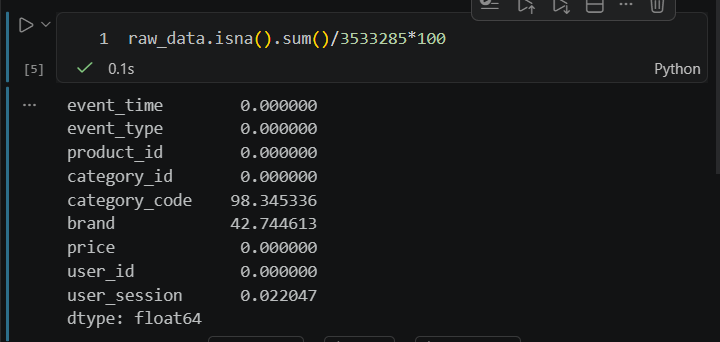
\includegraphics[width=0.9\textwidth]{IMG/NullCheck.png}
            \end{center}
        \end{column}
    \end{columns}
\end{frame}

\begin{frame}{2.2 Kiểm tra chất lượng dữ liệu thô (Phần 2)}
    \begin{columns}
        \begin{column}{0.5\textwidth}
            \textbf{3. Kiểm tra Trùng lặp (Duplication):}
            \begin{itemize}
                \item Hệ thống ghi nhận \textbf{5.2\%} các dòng bị trùng lặp hoàn toàn đến từng mili-giây.
                \item \textit{Nguyên nhân:} Việc người dùng click đúp (double-click) do lỗi mạng hoặc độ trễ giao diện.
            \end{itemize}
            \begin{center}
                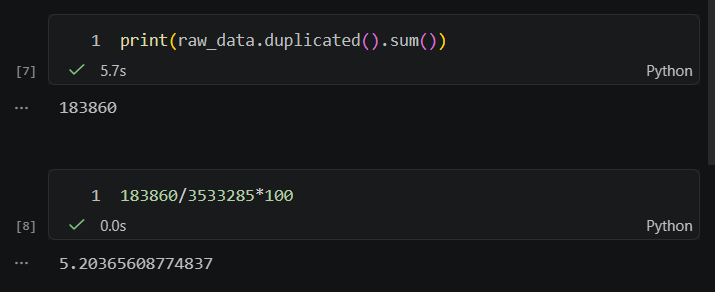
\includegraphics[width=0.9\textwidth]{IMG/DupCheck.png}
            \end{center}
        \end{column}
        
        \begin{column}{0.5\textwidth}
            \textbf{4. Kiểm tra Ngoại lệ (Outliers):}
            \begin{itemize}
                \item Cột \texttt{price} có xuất hiện các giá trị âm ($<0$) do lỗi hệ thống backend.
                \item Xuất hiện một số sản phẩm có giá cao bất thường (lên tới hàng ngàn USD) gây nhiễu cho mô hình.
            \end{itemize}
            \begin{center}
                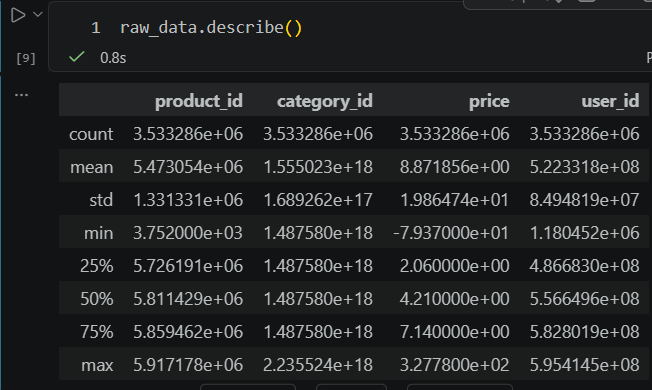
\includegraphics[width=0.9\textwidth]{IMG/Describe.png}
            \end{center}
        \end{column}
    \end{columns}
\end{frame}


\begin{frame}{2.3 Tiền xử lý - Giai đoạn 1: Làm sạch dữ liệu (Phần 1)}
    \begin{columns}
        \begin{column}{0.5\textwidth}
            \textbf{Xử lý trùng lặp và ngoại lệ:}
            \begin{itemize}
                \item \textbf{Loại bỏ trùng lặp:} Tiến hành loại bỏ hoàn toàn các dòng trùng lặp (Drop duplicates).
                \item \textbf{Xóa giá âm/0:} Các bản ghi có \texttt{price $\le$ 0} bị loại bỏ vì không mang ý nghĩa kinh doanh.
                \item \textbf{Giới hạn ngoại lệ (Winsorization):} Các mặt hàng có giá lớn hơn phân vị thứ 99 (99th percentile) được giới hạn lại để giảm tác động của nhiễu.
            \end{itemize}
        \end{column}
        \begin{column}{0.5\textwidth}
            \begin{center}
                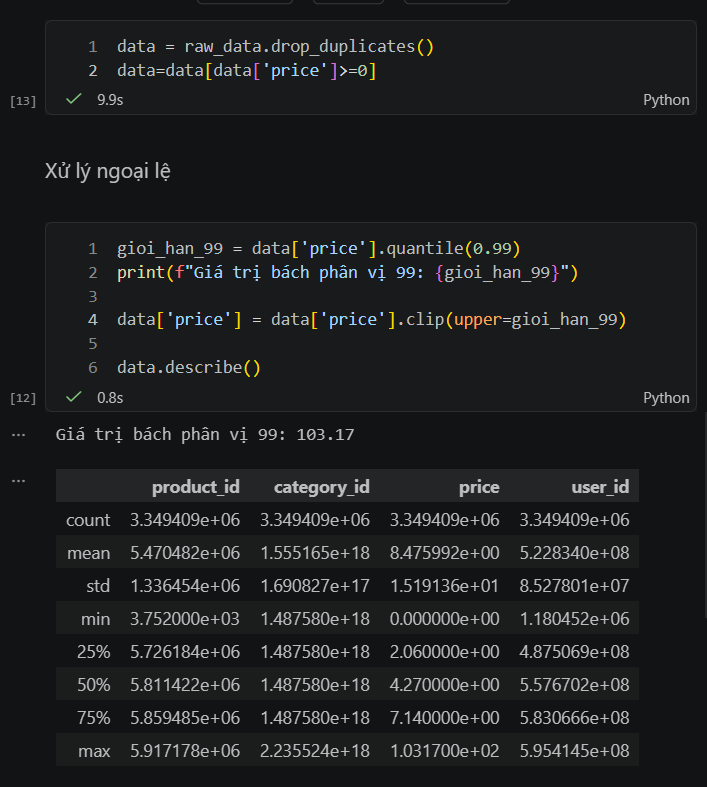
\includegraphics[width=\textwidth]{IMG/ETL1.png} \\
                \vspace{0.2cm}
                \scriptsize{\textit{Làm sạch dữ liệu thô}}
            \end{center}
        \end{column}
    \end{columns}
\end{frame}

\begin{frame}{2.3 Tiền xử lý - Giai đoạn 1: Làm sạch dữ liệu (Phần 2)}
    \begin{columns}
        \begin{column}{0.5\textwidth}
            \textbf{Xử lý dữ liệu thiếu \& Cột không đóng góp:}
            \begin{itemize}
                \item \textbf{Điền khuyết \texttt{brand}:} Thay vì xóa (sẽ mất 42\% traffic), giá trị \texttt{Null} được điền bằng \textit{"Unknown"}. (Sản phẩm "Không thương hiệu" cũng là đặc trưng hành vi).
                \item \textbf{Xóa cột nhiễu:} Xóa \texttt{category\_code} (khuyết 98\%) và \texttt{user\_id} (không giúp phân loại phiên).
                \item \textbf{Xử lý session rác:} Loại bỏ các dòng có \texttt{user\_session} bị Null (khoảng 2.2\%).
            \end{itemize}
        \end{column}
        \begin{column}{0.5\textwidth}
            \begin{center}
                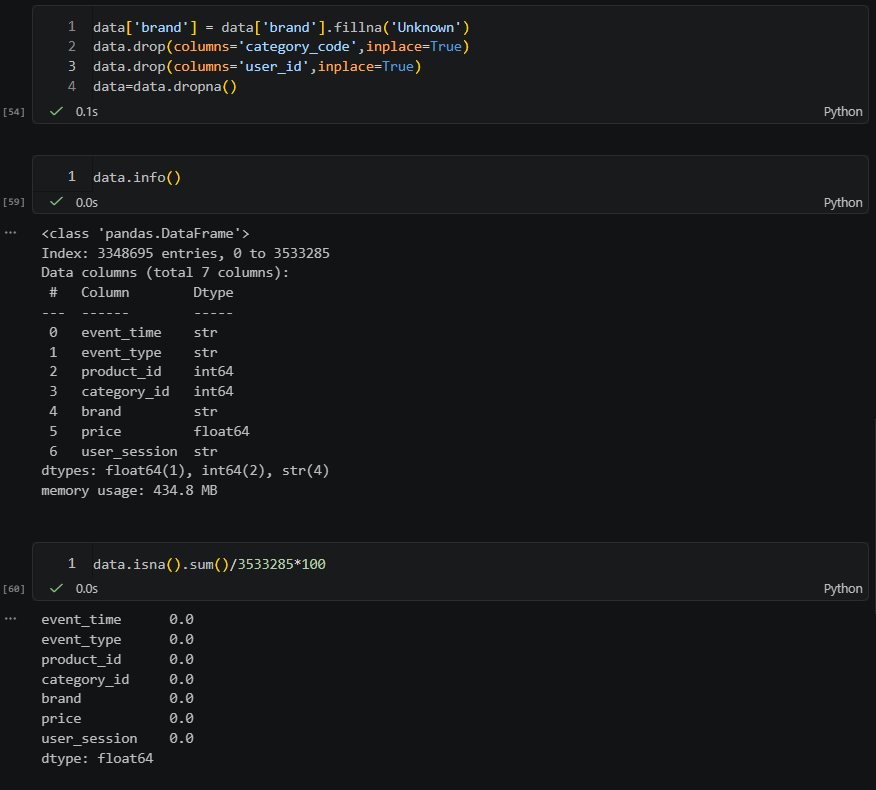
\includegraphics[width=\textwidth]{IMG/ETL2.png} \\
                \vspace{0.2cm}
                \scriptsize{\textit{Xử lý khuyết dữ liệu và cột không đóng góp}}
            \end{center}
        \end{column}
    \end{columns}
\end{frame}

\begin{frame}{2.4 Tiền xử lý - Giai đoạn 2: Trích xuất theo Phiên (Sessionization)}
    \begin{columns}
        \begin{column}{0.5\textwidth}
            \textbf{Tiên xử lý:}
            \begin{itemize}
                \item \textbf{Biến mục tiêu (Target):} Gán $Y=1$ nếu phiên có sự kiện \texttt{purchase}, ngược lại $Y=0$.
                \item \textbf{Xóa} toàn bộ sự kiện \texttt{purchase} khỏi tập huấn luyện.
             
            \end{itemize}
            \textbf{Tổng hợp đặc trưng:} 
                \begin{itemize}
                    \item \texttt{total\_views}, \texttt{total\_carts}
                    \item \texttt{session\_duration}
                    \item \texttt{unique\_products}, \texttt{avg\_price}, \texttt{max\_price}
                \end{itemize}
        \end{column}
        \begin{column}{0.5\textwidth}
            \begin{center}
                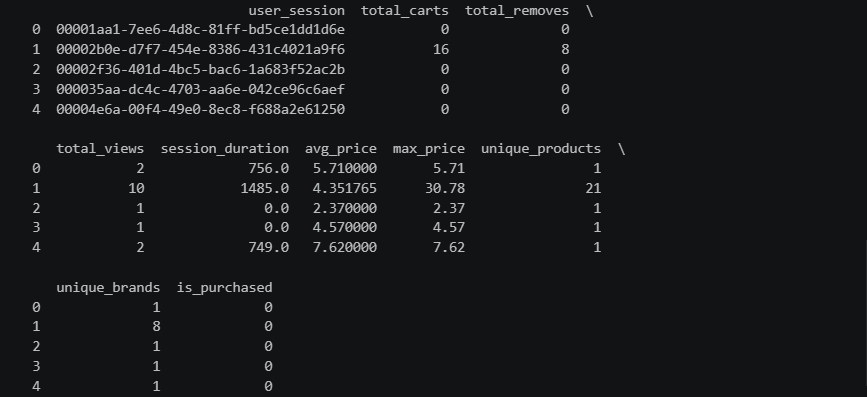
\includegraphics[width=0.9\textwidth]{IMG/ETL3.png}
                \vspace{0.2cm}
                
            \end{center}
        \end{column}
    \end{columns}
\end{frame}

% ==========================================
\section{3. Khám phá dữ liệu (EDA)}
% ==========================================

\begin{frame}{3.1 EDA: Phân bố nhãn (Class Imbalance)}
    \begin{columns}
        \begin{column}{0.5\textwidth}
            \begin{itemize}
                \item Dữ liệu mất cân bằng nhãn cực kỳ nghiêm trọng.
                \item Số lượng phiên \textbf{Không mua (0)} áp đảo hoàn toàn phiên \textbf{Có mua (1)}.
                \item Thách thức lớn cho các thuật toán Học máy cơ bản $\rightarrow$ Cần kỹ thuật lấy mẫu (Sampling) ở bước huấn luyện.
            \end{itemize}
        \end{column}
        \begin{column}{0.5\textwidth}
            \begin{center}
                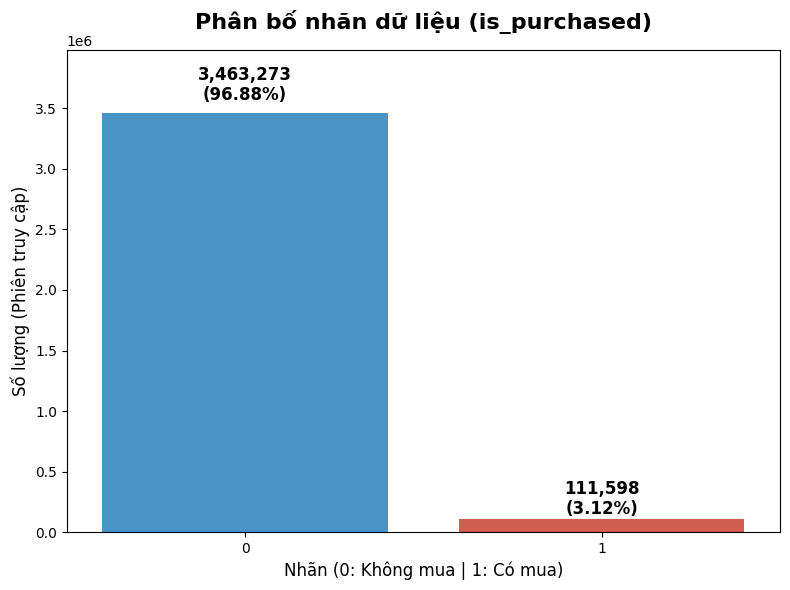
\includegraphics[width=0.9\textwidth]{IMG/phanbonhan.png}
            \end{center}
        \end{column}
    \end{columns}
\end{frame}

\begin{frame}{3.2 EDA: Phân bố đặc trưng}
    \begin{center}
        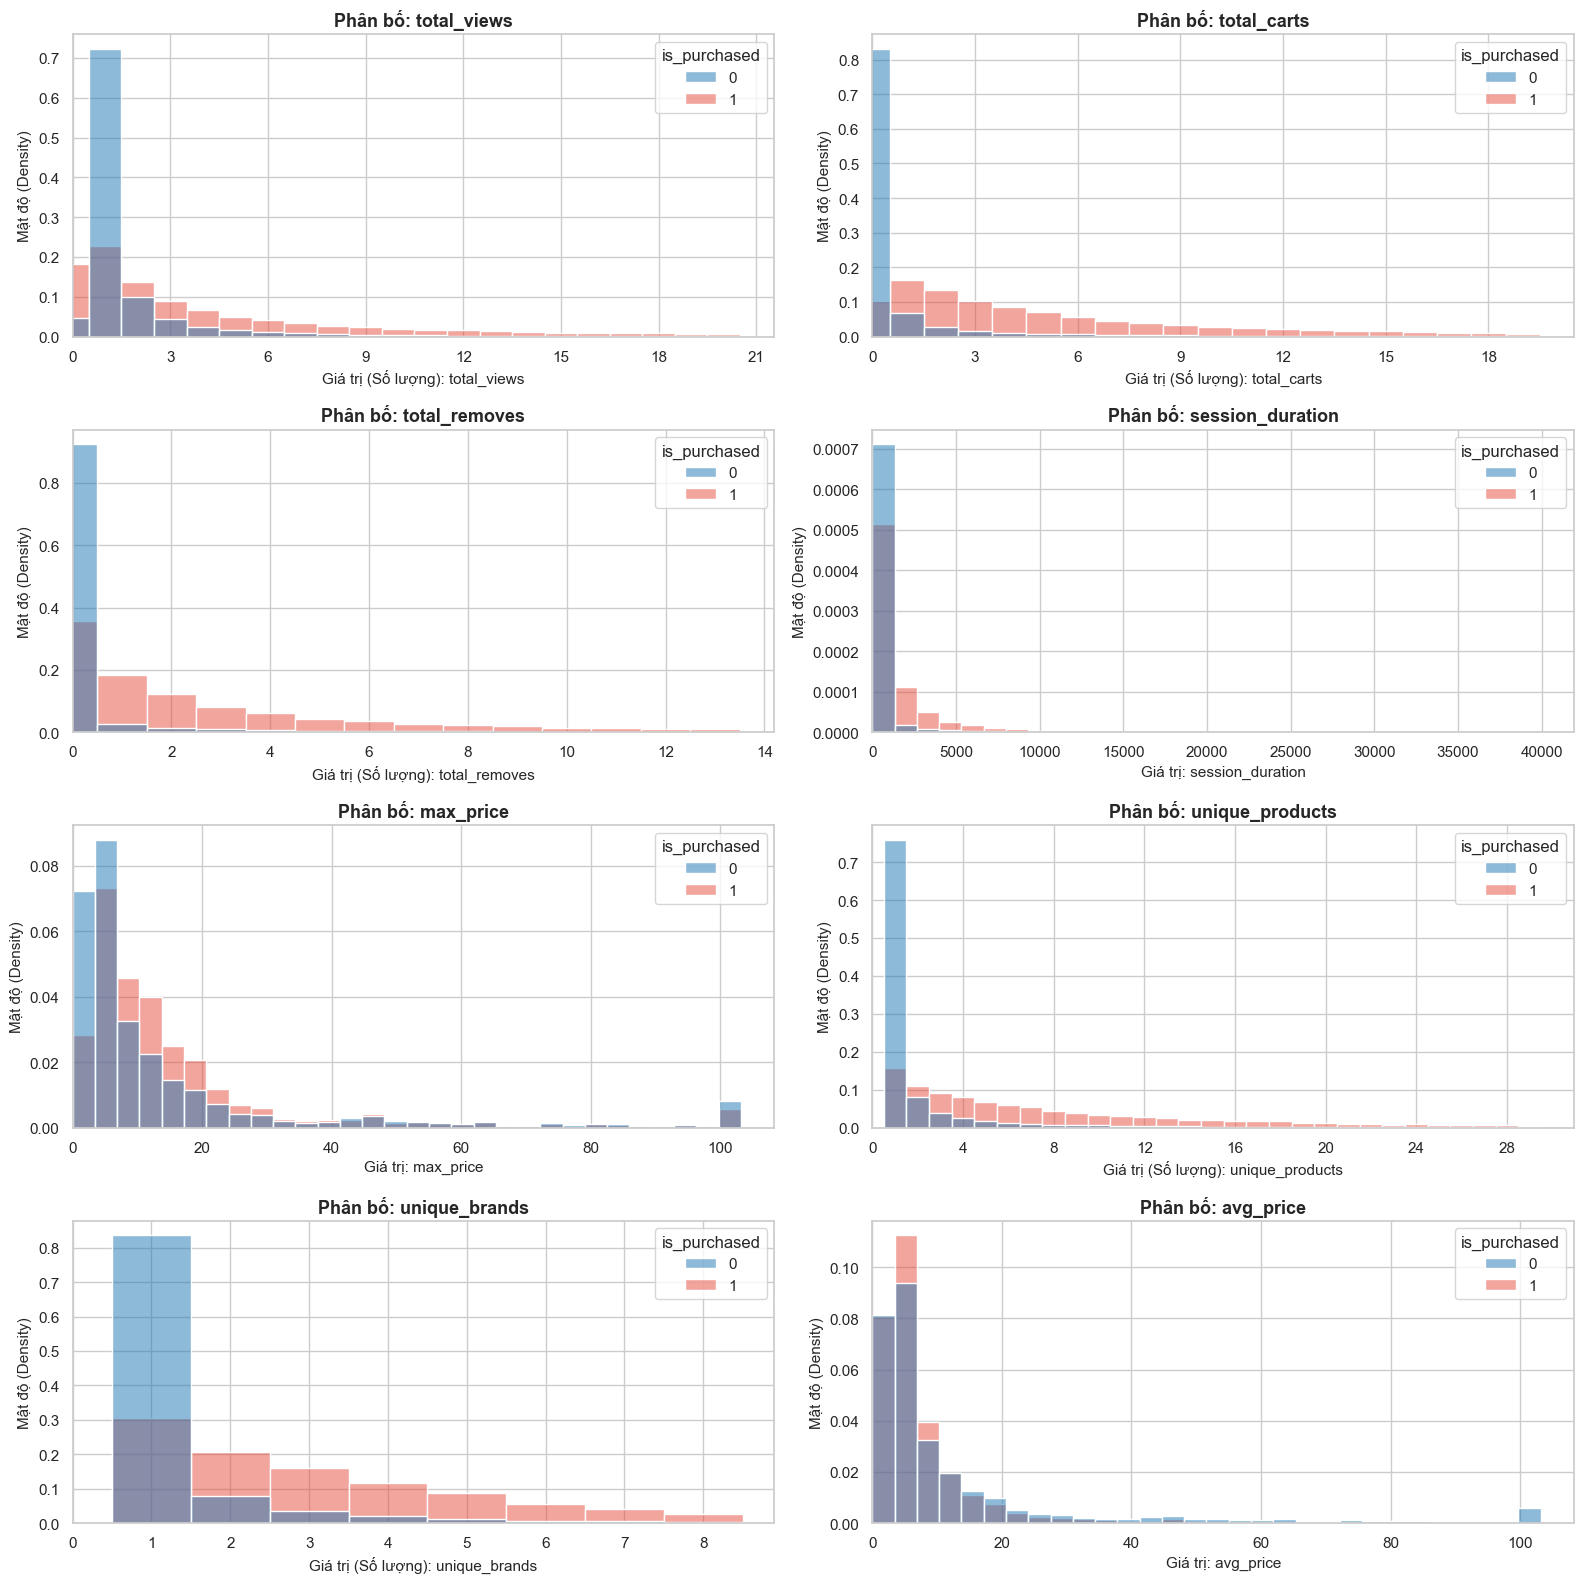
\includegraphics[width=0.5\textwidth]{IMG/feature_distributions.png}
    \end{center}
\end{frame}

\begin{frame}{3.2 EDA: Các Insight từ phân bố đặc trưng}
    \begin{itemize}
        \item \textbf{Insight 1 - Nhóm "Bounce" (Thoát trang nhanh):} Tập trung ở mốc 1 \texttt{view}, 0 giây. Là nhóm click nhầm, không có tương tác.
        \item \textbf{Insight 2 - Xóa khỏi giỏ không phải tín hiệu xấu:} Biểu đồ \texttt{total\_removes} của Lớp 1 trải dài. Điều này thể hiện sự so sánh, chọn lọc kỹ (Active Shopping) của người có ý định mua.
        \item \textbf{Insight 3 - Window Shopping:} Người mua hàng thường xem từ 2 đến 6 \texttt{unique\_products} trước khi chốt đơn.
        \item \textbf{Insight 4 - Nghịch lý Giá cả:} Phân bố \texttt{avg\_price} của hai Lớp chồng khít lên nhau. Giá tiền KHÔNG phải yếu tố phân loại ý định mua!
    \end{itemize}
\end{frame}

\begin{frame}{3.3 EDA: Tương quan giữa các đặc trưng}
    \begin{columns}
        \begin{column}{0.5\textwidth}
            \textbf{Insight Tương quan:}
            \begin{itemize}
                \item \textbf{Giỏ hàng là Vua:} \texttt{total\_carts} \& \texttt{total\_removes} tương quan dương cao nhất (0.34) với biến mục tiêu. \texttt{views} chỉ đạt 0.12.
                \item \textbf{Mức giá độc lập:} \texttt{avg\_price} có tương quan xấp xỉ 0 với nhãn $\rightarrow$ Sẽ bị loại bỏ khi đưa vào mô hình để giảm nhiễu.
                \item \textbf{Đa cộng tuyến:} \texttt{session\_duration} và \texttt{unique\_products} tương quan rất mạnh (0.84).
            \end{itemize}
        \end{column}
        \begin{column}{0.5\textwidth}
            \begin{center}
                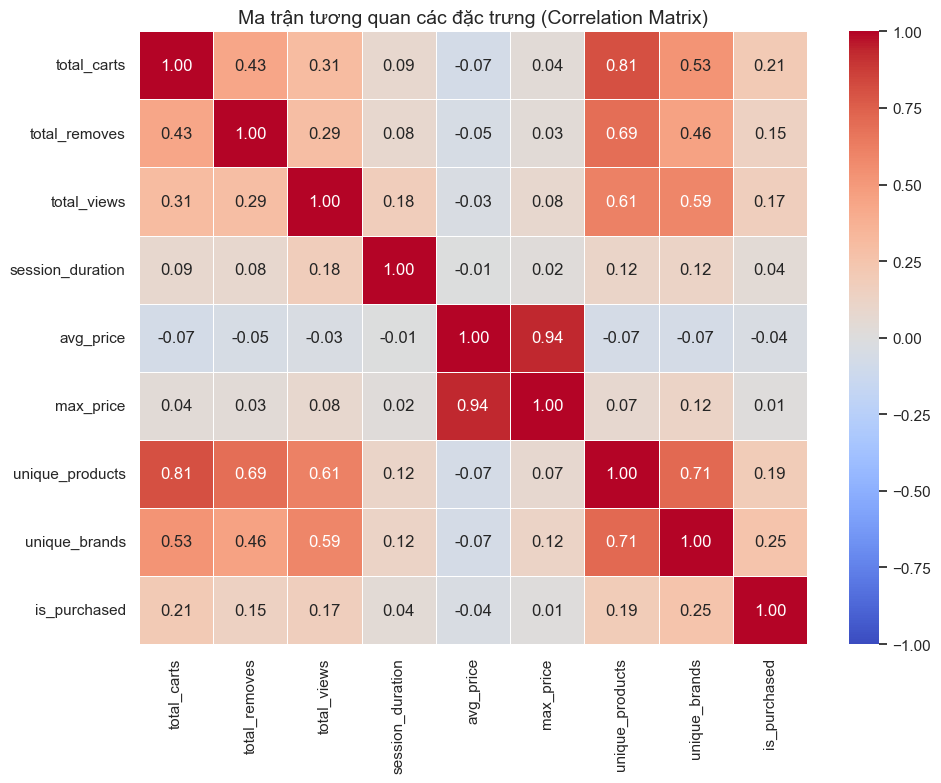
\includegraphics[width=\textwidth]{IMG/Corr.png}
            \end{center}
        \end{column}
    \end{columns}
\end{frame}

% ==========================================
\section{4. Huấn luyện mô hình}
% ==========================================

\begin{frame}{4.1 Chiến lược xây dựng mô hình}
    \textbf{Mục tiêu Đánh giá:} Tập trung tối ưu \textbf{F1-Score} và \textbf{Độ phủ (Recall)} nhằm không bỏ lọt khách hàng tiềm năng. \\
    \textbf{Feature Selection:} Bỏ \texttt{avg\_price} và \texttt{max\_price}.
    
    \vspace{0.3cm}
    \textbf{Chiến lược xử lý Mất cân bằng (Ensemble-based Undersampling):}
    \begin{itemize}
        \item Không Undersampling thông thường (gây mất mát thông tin Lớp 0).
        \item \textbf{Giải pháp:} Chia tập Lớp 0 thành 11 phần nhỏ. Ghép từng phần với toàn bộ tập Lớp 1 $\rightarrow$ Tạo 11 tập dữ liệu cân bằng.
        \item Huấn luyện 11 mô hình con và kết hợp kết quả (Voting/Averaging) $\rightarrow$ Giảm phương sai (Variance), tận dụng 100\% dữ liệu.
    \end{itemize}
\end{frame}

% ==========================================
\section{5. Kết quả và Đánh giá}
% ==========================================

\begin{frame}{5.1 Baseline Model \& Mô hình trước xử lý mất cân bằng}
    \begin{columns}
        \begin{column}{0.5\textwidth}
            \textbf{1. Baseline (Logistic Regression)} \\
            (Ngưỡng 0.73)
            \resizebox{\textwidth}{!}{
            \begin{tabular}{lccc}
                \toprule
                 & \textbf{Precision} & \textbf{Recall} & \textbf{F1-score} \\
                \midrule
                Lớp 0 & 0.98 & 0.95 & 0.97 \\
                \textbf{Lớp 1} & \textbf{0.24} & \textbf{0.49} & \textbf{0.32} \\
                \bottomrule
            \end{tabular}
            }
            \vspace{0.3cm}
            
            \textbf{2. LightGBM (Trước xử lý)} \\
            \resizebox{\textwidth}{!}{
            \begin{tabular}{lccc}
                \toprule
                 & \textbf{Precision} & \textbf{Recall} & \textbf{F1-score} \\
                \midrule
                Lớp 0 & 0.98 & 0.95 & 0.97 \\
                \textbf{Lớp 1} & \textbf{0.29} & \textbf{0.55} & \textbf{0.37} \\
                \bottomrule
            \end{tabular}
            }
        \end{column}
        
        \begin{column}{0.5\textwidth}
            \textbf{3. Cây quyết định (Trước xử lý)} \\
            \begin{center}
                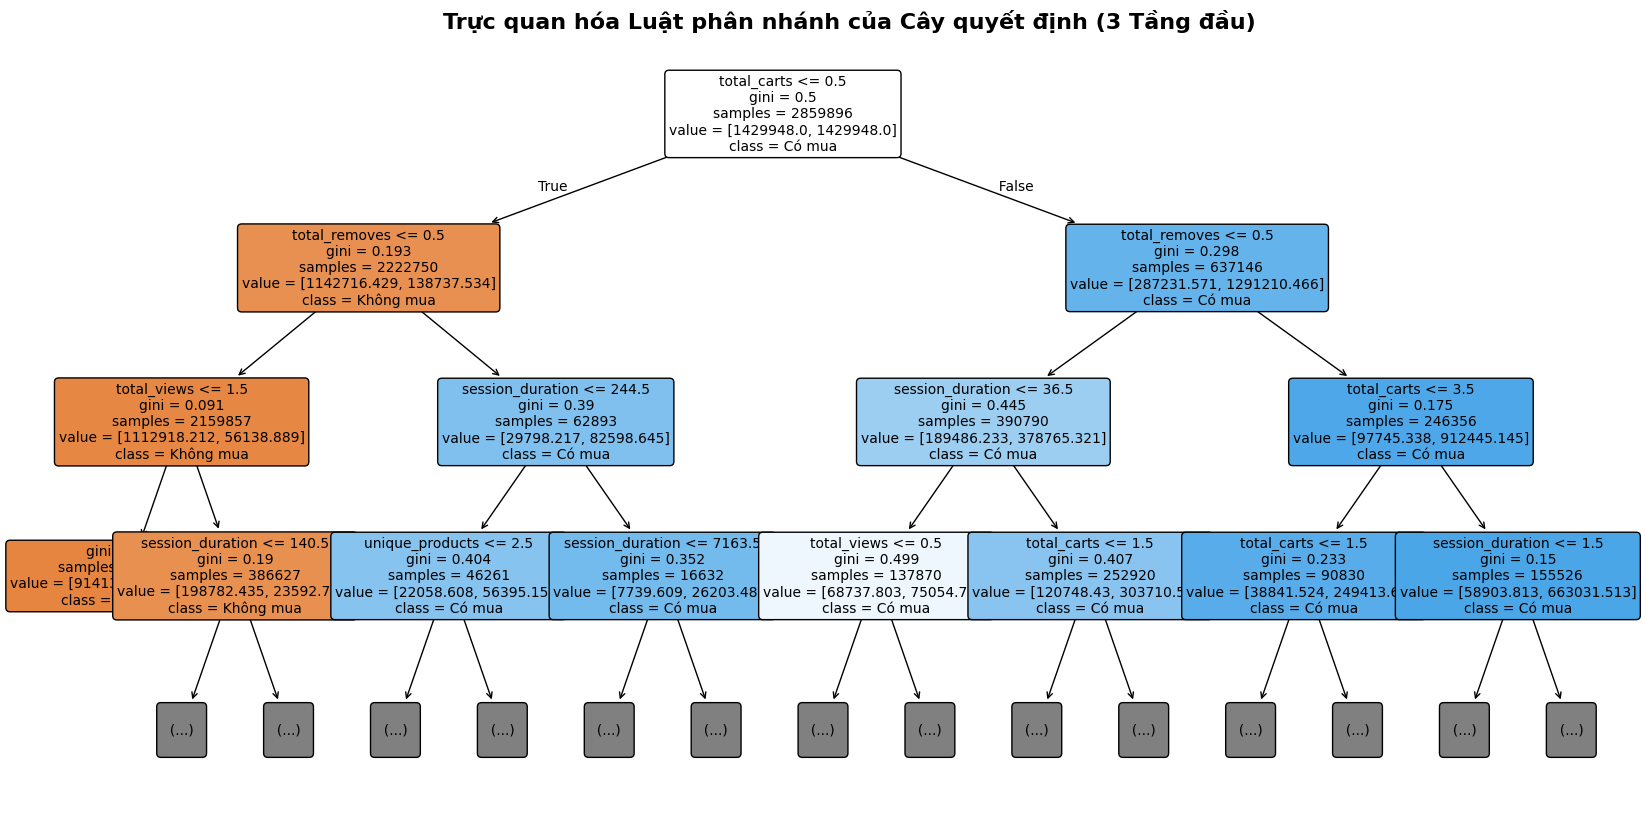
\includegraphics[width=0.8\textwidth]{IMG/cayquyetdinh.png}
                \resizebox{\textwidth}{!}{
                \begin{tabular}{lccc}
                    \toprule
                     & \textbf{Prec} & \textbf{Recall} & \textbf{F1} \\
                    \midrule
                    Lớp 1 & 0.27 & 0.52 & 0.35 \\
                    \bottomrule
                \end{tabular}
                }
            \end{center}
        \end{column}
    \end{columns}
\end{frame}

\begin{frame}{5.2 Hiệu năng Mô hình Sau khi áp dụng Ensemble}
    \textbf{1. Ensemble Cây quyết định (Random Forest + Bagging)} \\
    (Ngưỡng 0.88)
    \begin{table}[H]
        \centering
        \begin{tabular}{lccc}
            \toprule
             & \textbf{Precision} & \textbf{Recall} & \textbf{F1-score} \\
            \midrule
            Lớp 0 & 0.98 & 0.96 & 0.97 \\
            \textbf{Lớp 1} & \textbf{0.27} & \textbf{0.51} & \textbf{0.36} \\
            \bottomrule
        \end{tabular}
    \end{table}

    \textbf{2. Ensemble LightGBM (Mô hình tốt nhất được chọn)} \\
    \begin{table}[H]
        \centering
        \begin{tabular}{lccc}
            \toprule
             & \textbf{Precision} & \textbf{Recall} & \textbf{F1-score} \\
            \midrule
            Lớp 0 & 0.99 & 0.95 & 0.97 \\
            \textbf{Lớp 1} & \textbf{0.27} & \textbf{0.61} & \textbf{0.37} \\
            \bottomrule
        \end{tabular}
    \end{table}
\end{frame}

\begin{frame}{5.3 Đánh giá Tổng thể (Trade-off Phân tích)}
    \begin{itemize}
        \item \textbf{Sức mạnh nội tại:} Ngay từ đầu, LightGBM đã áp đảo Cây quyết định (F1: 0.37 so với 0.35), chứng minh ưu thế của Tăng cường độ dốc (Gradient Boosting).
        \item \textbf{Hiệu năng Ensemble (Sự đánh đổi):}
        \begin{itemize}
            \item Precision giảm nhẹ $2\%$ (từ 0.29 $\rightarrow$ 0.27).
            \item \textbf{Recall tăng vọt $6\%$} (từ 0.55 $\rightarrow$ 0.61). F1-Score giữ vững.
        \end{itemize}
        \item \textbf{Ý nghĩa Kinh doanh:} Với 22.320 giao dịch Lớp 1 trong tập test, Recall tăng 6\% giúp bắt trúng thêm $\sim$\textbf{1.339 khách hàng tiềm năng}. Vì chi phí Retargeting (Email/Push) rất rẻ, việc hi sinh 2\% chuẩn xác để tăng độ phủ mang lại \textbf{Lợi nhuận ròng (Net Profit) vượt trội}.
    \end{itemize}
\end{frame}

% ==========================================
\section{6. Khuyến nghị và Hướng phát triển}
% ==========================================

\begin{frame}{6.1 Khuyến nghị Ra quyết định (Actionable Insights)}
    \begin{enumerate}
        \item \textbf{Targeted Retargeting:} Ngừng chạy Ads đại trà. Chỉ tập trung ngân sách cho tập khách hàng được gán \textbf{Nhãn 1} $\rightarrow$ Giảm CAC, tăng vọt ROAS.
        \item \textbf{Smart Vouchering (Phân phối mã giảm giá):}
        \begin{itemize}
            \item Xác suất > 90\%: Không cấp Voucher (Bảo vệ lợi nhuận).
            \item Xác suất 70\%-90\%: Kích hoạt Pop-up Voucher 15 phút (Ép FOMO).
            \item Xác suất < 50\%: Gợi ý đọc Blog để lấy Email.
        \end{itemize}
        \item \textbf{Real-time CS Intervention:} Bật cảnh báo cho nhân viên CSKH khi khách Nhãn 1 dừng ở trang Checkout quá 3 phút.
        \item \textbf{Dynamic UI/UX:} Tự động ẩn banner, đưa nút thanh toán ra giữa màn hình với nhóm có ý định mua cao.
    \end{enumerate}
\end{frame}

\begin{frame}{6.2 Rủi ro \& Hạn chế (Risks \& Limitations)}
    \textbf{1. Rủi ro Kinh doanh:}
    \begin{itemize}
        \item Mặc dù Recall cao, Precision vẫn ở mức 27\% (Có False Positives). Khuyến nghị này \textbf{chỉ an toàn với Marketing chi phí thấp} (Email, Push). KHÔNG dùng cho Telesales/Voucher quá lớn.
        \item Nguy cơ thao túng thuật toán (Voucher Abuse) $\rightarrow$ Cần Randomization và Rate Limiting.
        \item \textbf{Bắt buộc:} Cần chạy \textbf{A/B Testing} trước khi Roll-out toàn bộ.
    \end{itemize}
    
    \textbf{2. Hạn chế Kỹ thuật:}
    \begin{itemize}
        \item Mô hình đang đánh giá rời rạc theo từng Phiên (Session), chưa nối được hành trình dài hạn (Cross-device/Long-term Journey).
        \item Bỏ qua tính tuần tự (Sequential) của chuỗi Click chuột.
    \end{itemize}
\end{frame}


\end{document}